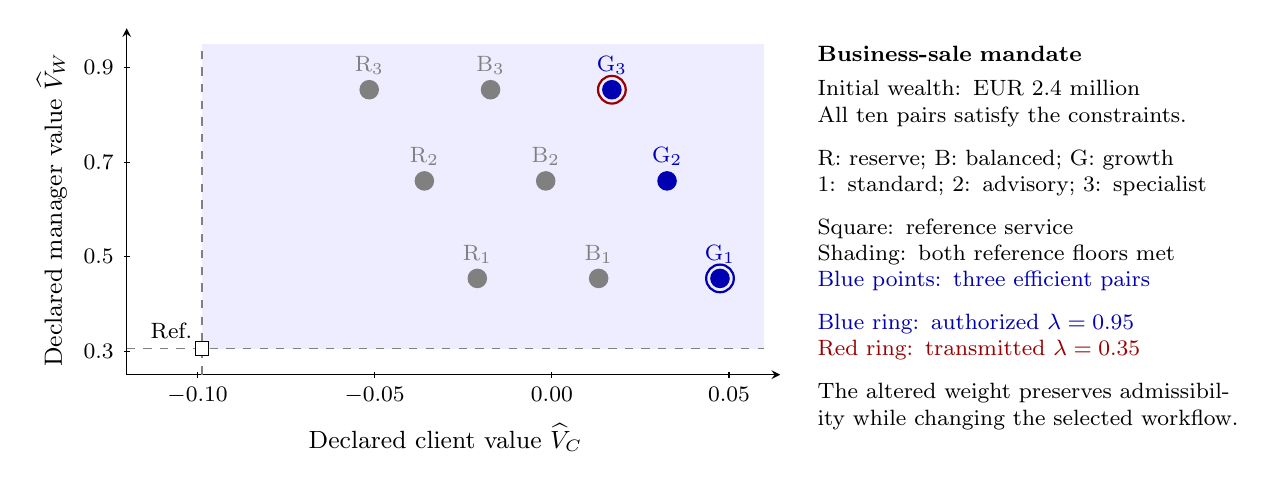
\begin{tikzpicture}[font=\small,>=stealth]
  \fill[blue!7] (0.95662,0.33100) rectangle (8.1,4.2);
  \draw[->] (0,0) -- (8.3,0);
  \draw[->] (0,0) -- (0,4.4);
  \draw[dashed,gray] (0.95662,0) -- (0.95662,4.2);
  \draw[dashed,gray] (0,0.33100) -- (8.1,0.33100);
  \draw (0.90000,0.04) -- (0.90000,-0.04) node[below,font=\footnotesize] {$ -0.10 $};
  \draw (3.15000,0.04) -- (3.15000,-0.04) node[below,font=\footnotesize] {$ -0.05 $};
  \draw (5.40000,0.04) -- (5.40000,-0.04) node[below,font=\footnotesize] {$ 0.00 $};
  \draw (7.65000,0.04) -- (7.65000,-0.04) node[below,font=\footnotesize] {$ 0.05 $};
  \draw (0.04,0.30000) -- (-0.04,0.30000) node[left,font=\footnotesize] {$ 0.3 $};
  \draw (0.04,1.50000) -- (-0.04,1.50000) node[left,font=\footnotesize] {$ 0.5 $};
  \draw (0.04,2.70000) -- (-0.04,2.70000) node[left,font=\footnotesize] {$ 0.7 $};
  \draw (0.04,3.90000) -- (-0.04,3.90000) node[left,font=\footnotesize] {$ 0.9 $};
  \node[below] at (4.05,-0.5) {Declared client value $\widehat V_C$};
  \node[rotate=90] at (-0.95,2.1) {Declared manager value $\widehat V_W$};
  \node[circle,fill=gray,inner sep=2.5pt] at (5.32181,2.46100) {};
  \node[above=2pt,text=gray,font=\footnotesize] at (5.32181,2.46100) {$\mathrm{B}_2$};
  \node[circle,fill=gray,inner sep=2.5pt] at (4.62126,3.61900) {};
  \node[above=2pt,text=gray,font=\footnotesize] at (4.62126,3.61900) {$\mathrm{B}_3$};
  \node[circle,fill=gray,inner sep=2.5pt] at (5.99424,1.22260) {};
  \node[above=2pt,text=gray,font=\footnotesize] at (5.99424,1.22260) {$\mathrm{B}_1$};
  \node[circle,fill=blue!70!black,inner sep=2.5pt] at (6.86274,2.46100) {};
  \node[above=2pt,text=blue!70!black,font=\footnotesize] at (6.86274,2.46100) {$\mathrm{G}_2$};
  \node[circle,fill=blue!70!black,inner sep=2.5pt] at (6.16219,3.61900) {};
  \node[above=2pt,text=blue!70!black,font=\footnotesize] at (6.16219,3.61900) {$\mathrm{G}_3$};
  \draw[red!60!black,thick] (6.16219,3.61900) circle[radius=5pt];
  \node[circle,fill=blue!70!black,inner sep=2.5pt] at (7.53517,1.22260) {};
  \node[above=2pt,text=blue!70!black,font=\footnotesize] at (7.53517,1.22260) {$\mathrm{G}_1$};
  \draw[blue!70!black,thick] (7.53517,1.22260) circle[radius=5pt];
  \node[rectangle,draw,fill=white,inner sep=2.5pt] at (0.95662,0.33100) {};
  \node[above left,font=\footnotesize] at (0.95662,0.33100) {Ref.};
  \node[circle,fill=gray,inner sep=2.5pt] at (3.78088,2.46100) {};
  \node[above=2pt,text=gray,font=\footnotesize] at (3.78088,2.46100) {$\mathrm{R}_2$};
  \node[circle,fill=gray,inner sep=2.5pt] at (3.08033,3.61900) {};
  \node[above=2pt,text=gray,font=\footnotesize] at (3.08033,3.61900) {$\mathrm{R}_3$};
  \node[circle,fill=gray,inner sep=2.5pt] at (4.45330,1.22260) {};
  \node[above=2pt,text=gray,font=\footnotesize] at (4.45330,1.22260) {$\mathrm{R}_1$};
  \node[anchor=north west,align=left,text width=5.4cm,font=\footnotesize] at (8.65,4.3)
    {\textbf{Business-sale mandate}\\[3pt]
     Initial wealth: EUR 2.4 million\\
     All ten pairs satisfy the constraints.\\[6pt]
     R: reserve; B: balanced; G: growth\\
     1: standard; 2: advisory; 3: specialist\\[6pt]
     Square: reference service\\
     Shading: both reference floors met\\
     \textcolor{blue!70!black}{Blue points: three efficient pairs}\\[6pt]
     \textcolor{blue!70!black}{Blue ring: authorized $\lambda=0.95$}\\
     \textcolor{red!60!black}{Red ring: transmitted $\lambda=0.35$}\\[6pt]
     The altered weight preserves admissibility while changing the selected workflow.};
\end{tikzpicture}
